\chapter{\acl{hrc} System}
\label{chapter:hrc_system}

\textcolor{red}{needs a new chapter introduction}
% This chapter covers a review of the experimental infrastructure including relevant hardware and software tools used while developing the final solution.

\section{System Architecture \textcolor{red}{(LARCC, ROS-based framework)}}

The experimental part of this thesis was developed using the setup available at the Laboratory for Automation and Robotics (LAR) located in the Department of Mechanical Engineering at the University of Aveiro. This setup was designed to meet the requirements of the AUGMANITY mobilizing project\footnote{AUGMANITY website: \url{https://www.augmanity.pt}} and it contains an UR10e collaborative robot and multiple cameras, including the Orbbec Astra Pro RGBD camera which was utilized.

\begin{figure}[h]
\centerline{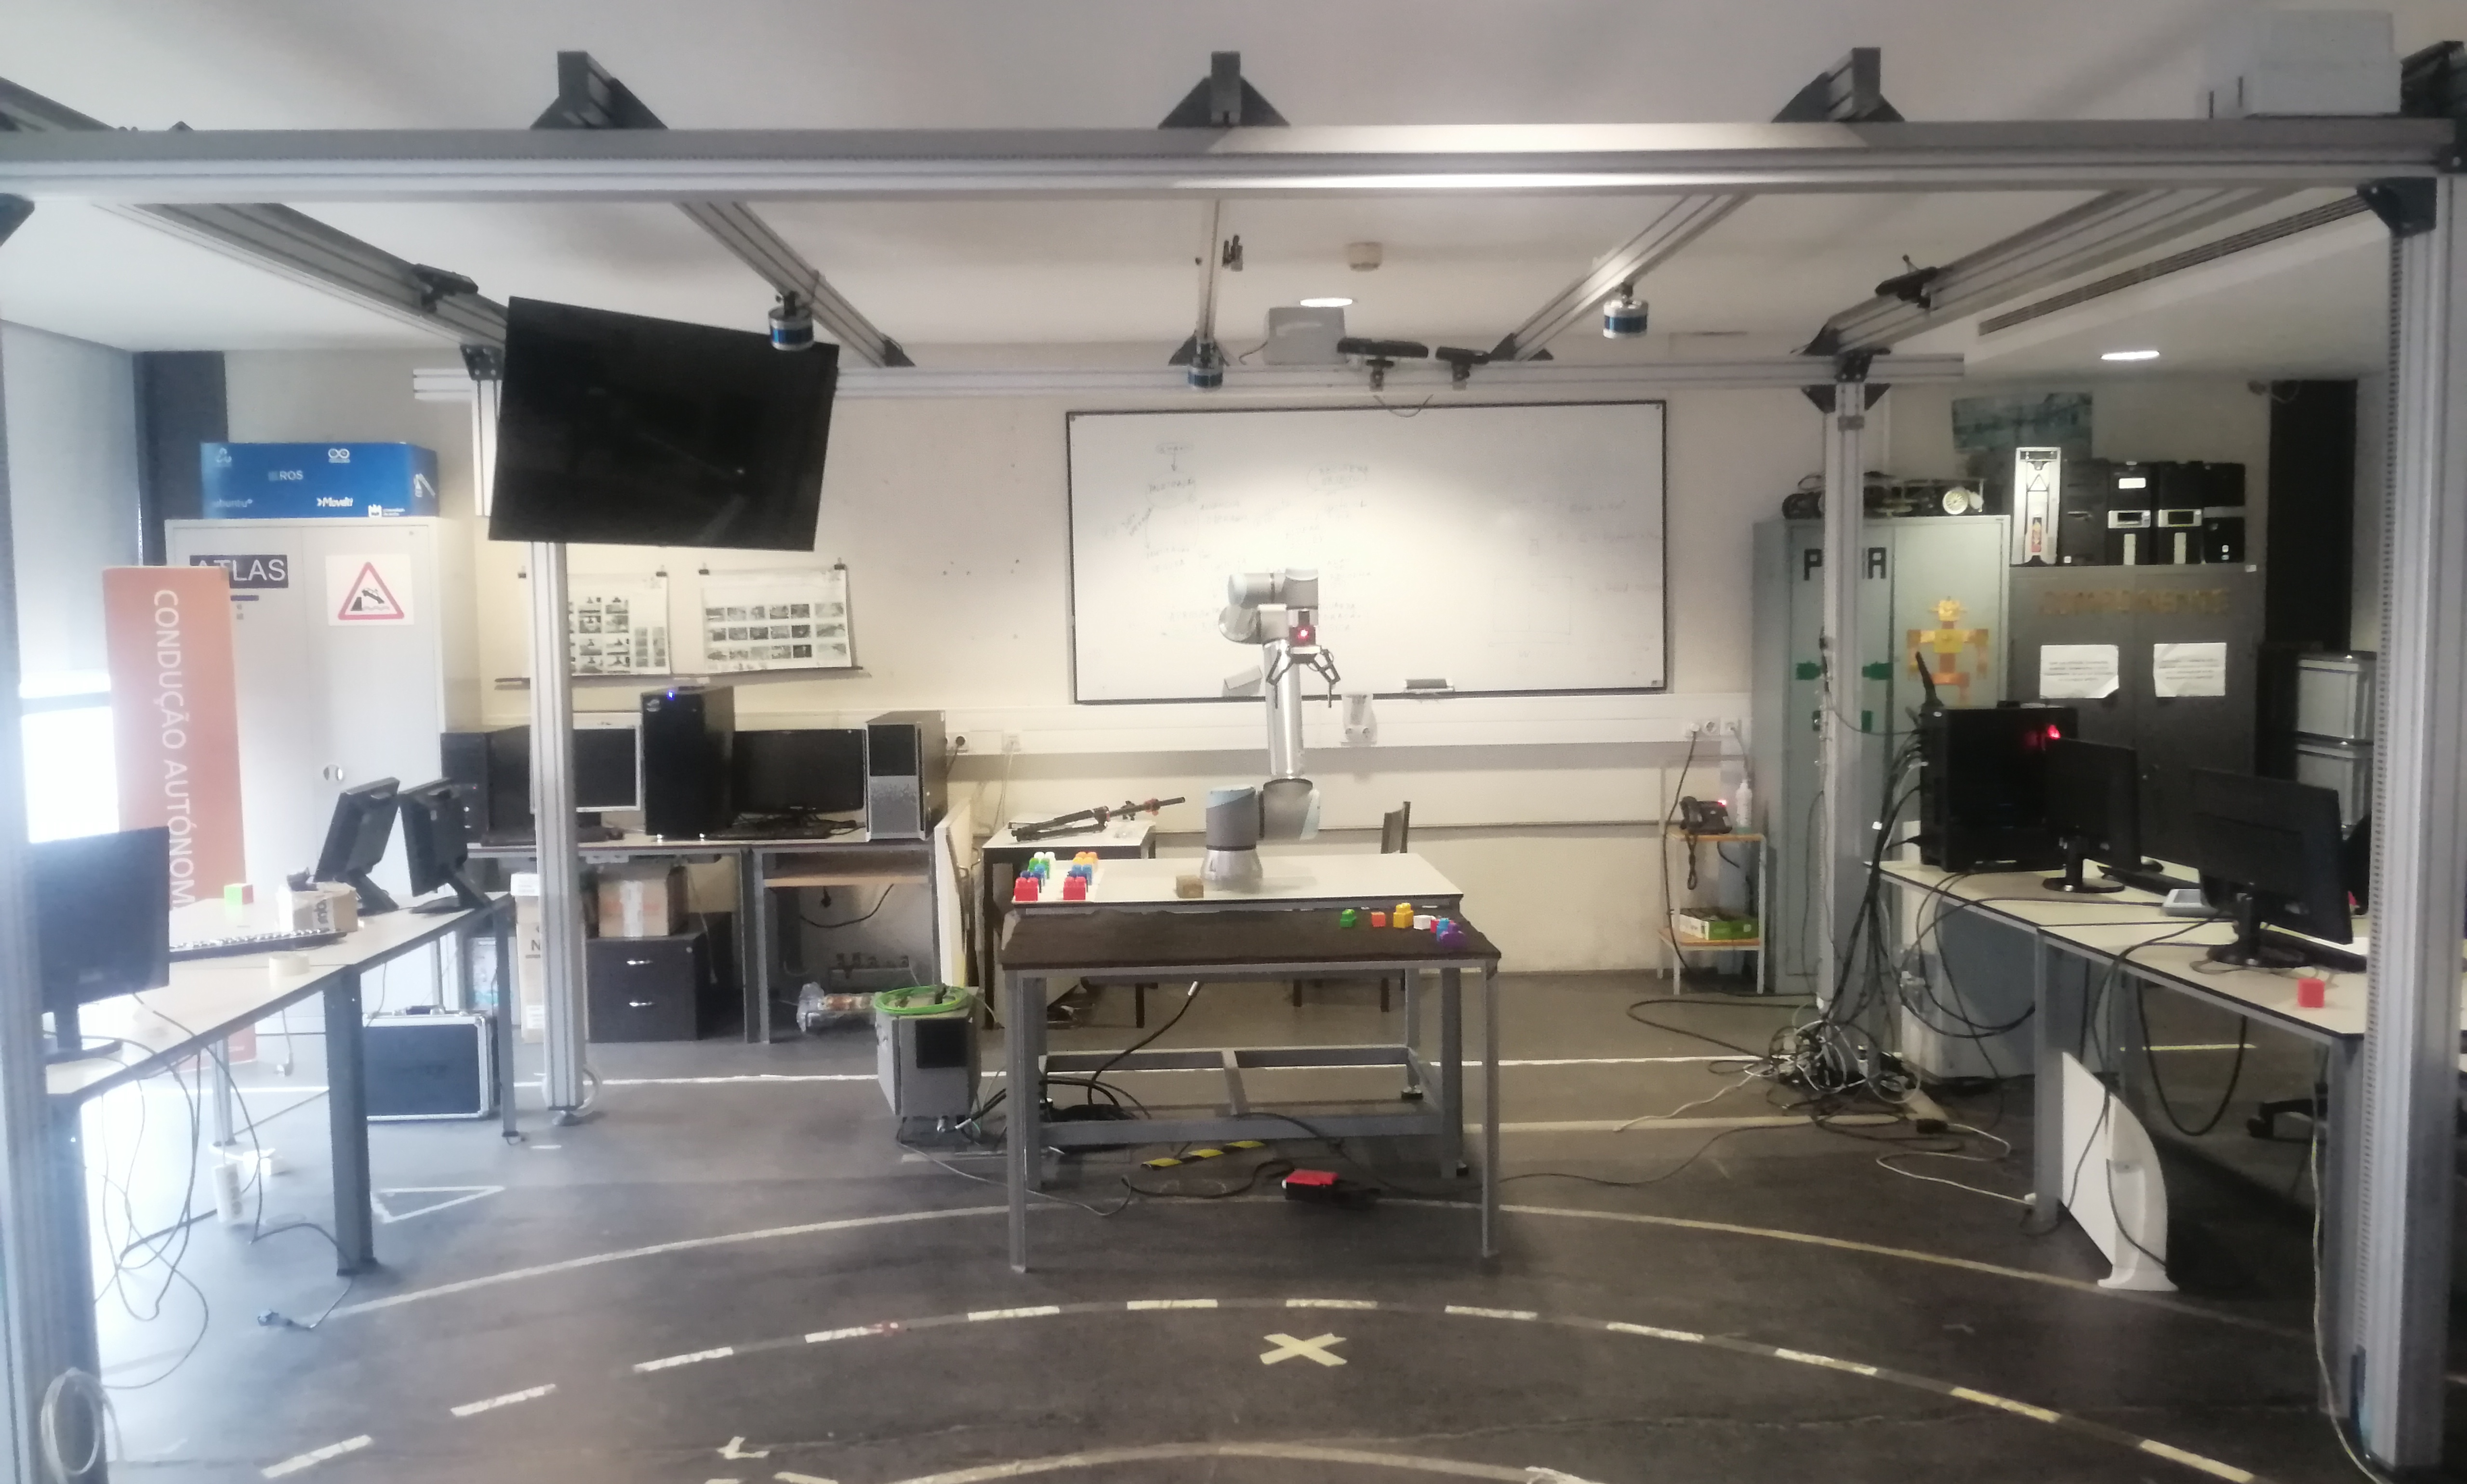
\includegraphics[height=3.2in]{figs/setup2.jpg}}
\caption[setup]{LAR hardware setup}
\label{fig:ur10e}
\end{figure}

\subsection{\acf{ros}}

\acs{ros}\cite{ROS2}\footnote{\acs{ros} 1 documentation: \url{https://wiki.ros.org}}\footnote{\acs{ros} 2 documentation: \url{https://docs.ros.org/en/humble}} is an open-source collection of tools and software libraries used to develop a robotics application. Its main features are:

\begin{itemize}
    \item \textbf{message broker}: every process in the project is a node in the \acs{ros} network and communicates with the other nodes mainly through topics (asynchronous publish/subscribe streaming of data) or services (synchronous RPC-style communication);
    \item \textbf{code reuse}: executables and packages are written to be as independent as possible, making the developer able to reuse them in another project;
    \item \textbf{rich ecosystem}: there are several open-source packages available to the developer that can be easily integrated;
    \item \textbf{scalability}: given that the nodes are so loosely coupled, it allows for node distribution;
    \item \textbf{language independence}: nodes can be written in any language since communication is established through well-defined objects;
    \item \textbf{data visualization}: there are tools to visualize the data in real-time, such as Rviz;
    \item \textbf{simulator support}: \acs{ros} has support for simulators with Gazebo being the most common;
    \item \textbf{hardware abstraction}: contains driver packages to deal with some hardware devices;
\end{itemize}

In this work, \acs{ros} is used to establish communication throughout all of the infrastructure. This makes it easier to integrate with previously developed software for the robot and set up the necessary drivers both for the robot and the camera. Additionally, Rviz is used to help visualize the functioning of the system.

\subsection{Perception System \textcolor{red}{(Orbbec Astra Pro, OpenCV)}}

\subsubsection{Orbbec Astra Pro}

Orbbec Astra Pro is an RGBD camera developed by Orbbec Technologies. It is frequently used in computer vision and robotics for tasks such as face recognition, gesture recognition, human body tracking, three-dimensional measurement, environment perception, and three-dimensional map reconstruction\cite{AstraPro}. In this work, the camera is placed above the environment facing down capturing both color and depth real-time images.

\begin{figure}[h]
\centerline{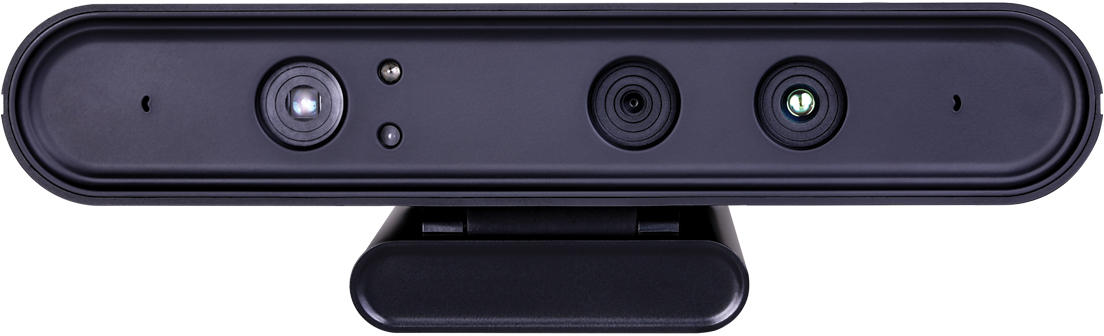
\includegraphics[height=1.2in]{figs/Astra.jpg}}
\caption[Orbbec Astra Pro]{Orbbec Astra Pro \cite{AstraPro}}
\label{fig:orbbec_astra_pro}
\end{figure}

\subsection{Manipulator Arm Control \textcolor{red}{(UR10e cobot, Robotiq gripper, Moveit)}}

\subsubsection{UR10e Robot}

UR10e is a collaborative robot model developed by Universal Robots focused on versatility. It allows for payloads up to 12.5 kg and has a reach of 1300mm being suitable for tasks such as machine tending, palletizing, and packaging\cite{UR10e}. The one used in this work is equipped with a \textcolor{red}{(missing gripper model)} gripper.

\begin{figure}[h]
\centerline{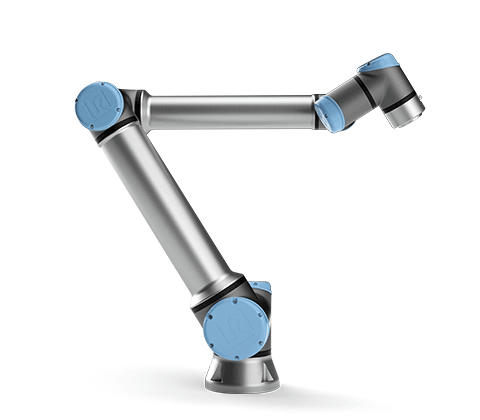
\includegraphics[height=2.5in]{figs/UR10e.png}}
\caption[UR10e]{UR10e collaborative robot \cite{UR10e_image} \textcolor{red}{(missing gripper image)}}
\label{fig:ur10e}
\end{figure}

\subsubsection{MoveIt}

MoveIt\footnote{MoveIt documentation: \url{https://ros-planning.github.io/moveit_tutorials}} is a widely-used open-source framework for robotics applications involving motion planning, manipulation, 3D perception, kinematics, control, navigation, and collision checking. MoveIt is implemented on top of ROS taking advantage of the latter's features such as the messaging and build systems as well as standard tools such as ROS Visualizer (Rviz) and the ROS robot format (URDF).

In this work, the MoveIt framework is used to plan and execute the robot arm movements with OMPL, an open-source motion planning library used by MoveIt for motion planning tasks.

\subsection{Computational Systems \textcolor{red}{(DeepLAR, Computador Central, TensorFlow)}}

\subsubsection{Tensorflow}

Tensorflow\footnote{Tensorflow documentation: \url{https://www.tensorflow.org/api_docs}} is a platform that can be used for all steps of a machine learning project. Its main features are:
\begin{itemize}
    \item \textbf{prepare data}: load data, data pre-processing and data augmentation;
    \item \textbf{build models}: design and train custom models with little code or use pre-trained ones (transfer learning);
    \item \textbf{deploy models}: helps using models in different platforms such as locally, in the cloud, in a browser, or in mobile;
    \item \textbf{implement MLOps}: run models in production, tracking their performance and identifying issues.
\end{itemize}

In this work, Tensorflow is used to design and train the machine learning models.

\section{Methodologies/Research Methods}

\subsection{Knowledge-Based Systems \textcolor{red}{(Experta)}}

\subsection{Keypoints Detection Frameworks \textcolor{red}{(OpenPose, OpenPifPaf, MediaPipe)}}
\label{subsection:keypointdetection}

This section reviews OpenPose and OpenPifPaf which are two projects containing models to detect key points in images, such as the human skeleton joints.

\subsubsection{OpenPose}

OpenPose\cite{Cao2021,Simon2017,Cao2018,Wei2016}\footnote{OpenPose documentation: \url{https://cmu-perceptual-computing-lab.github.io/openpose}} is an open-source project that aims to detect key points in the human body, face, hands, and feet from images. Its main features are:

\begin{itemize}
    \item 2D real-time key point detection based on the body/foot, the hand, or the face of multiple people;
    \item 3D real-time key point detection based on images from multiple cameras of one person;
    \item estimation of camera calibration parameters;
    \item single-person tracking.
\end{itemize}

OpenPose can be used through the command-line or using an API for Python or C++.

\begin{figure}[h]
\centerline{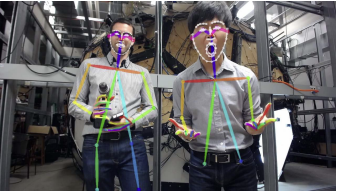
\includegraphics[height=1.55in]{figs/openpose.jpeg}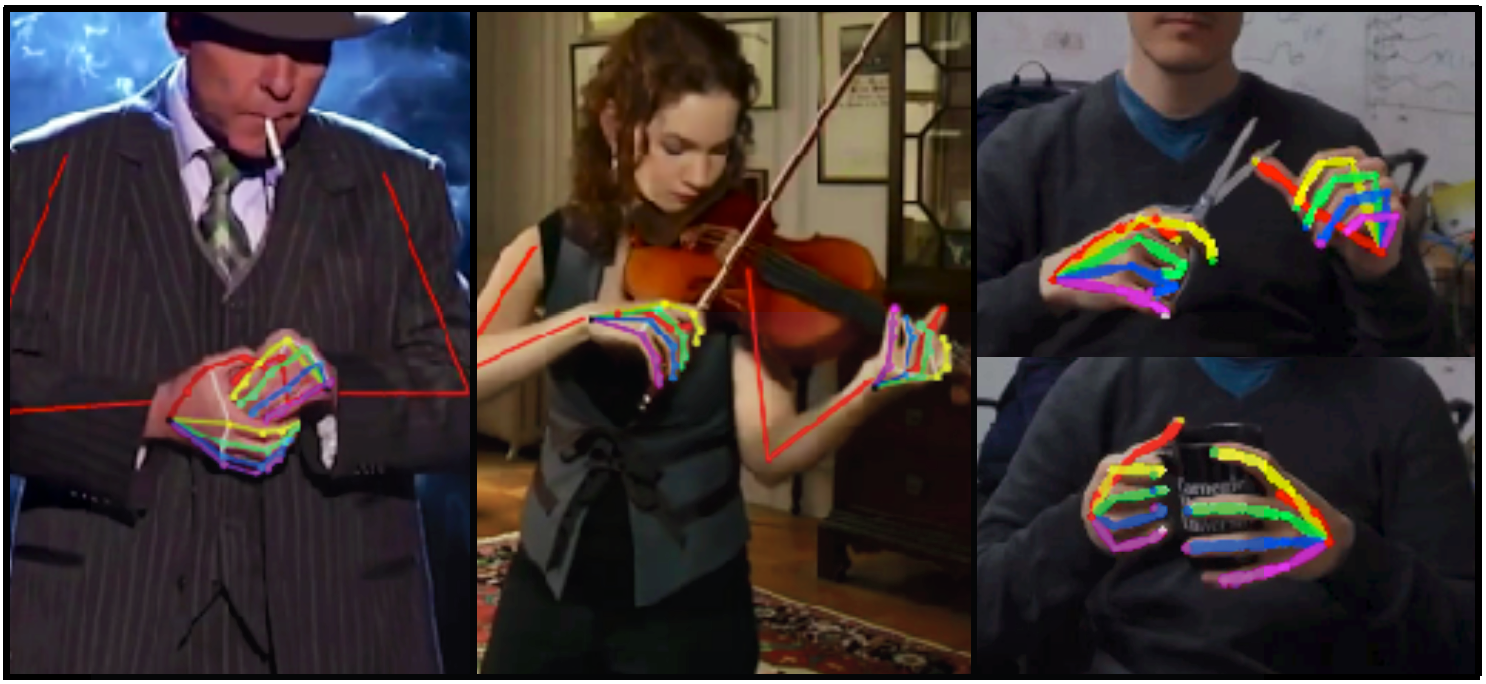
\includegraphics[height=1.55in]{figs/openpose2.PNG}}
\caption[OpenPose Examples]{OpenPose Examples \cite{Cao2021,Simon2017}}
\label{openpose}
\end{figure}

\subsubsection{OpenPifPaf}

OpenPifPaf\cite{Kreiss2021,Kreiss2019}\footnote{OpenPifPaf documentation: \url{https://openpifpaf.github.io}} is an open-source project that aims to detect, associate and track semantic key points. Detecting human joints is an example of its usage but it is also able to generalize this detection to other classes such as cars and animals. It can be installed as a python package which can then be imported.

\begin{figure}[h]
\centerline{\includegraphics[height=1.8in]{figs/openpifpaf.jpeg}}
\caption[OpenPifPaf Example]{OpenPifPaf Example \cite{Kreiss2021}}
\label{openpifpaf}
\end{figure}

\subsubsection{MediaPipe}

\subsection{Convolutional Neural Networks}

\subsection{Transformer Neural Networks}
\label{subsection:transformer_neural_networks}

Transformer Neural Networks consist of a new kind of neural network architecture that aims to solve tasks involving sequence data such as those in natural language processing. They were initially proposed in the "Attention Is All You Need" paper published by Google Research in 2017\cite{Vaswani2017} and proceeded to surpass several established architectures in numerous tasks using attention mechanisms that identify complex relationships between elements in the input sequence.

According to \textcolor{red}{https://learning.oreilly.com/library/view/deep-learning-with/9781803232911/}, the transformer's architectures are built upon 4 core concepts: positional encoding, attention, self-attention, and multi-head (self-)attention.

\subsubsection{Positional encoding}

RNNs are able to work with sequences given that the tokens are processed sequentially. However, this approach comes with the disadvantage of the model having greater difficulty in analyzing long sequences, since important data might be forgotten. Transformers address this issue by using positional encoding, assigning a unique number to each token representing its position in the input sequence. This enables the transformer to learn the significance of each token's position.

\subsubsection{Attention}

Attention is a concept that consists in measuring the relative importance of the input tokens to the output tokens. It was initially designed to facilitate language translation given that, when translating text from one language to the other, each word in the output can be influenced by multiple words from the input, and it became a key idea behind the transformer's architecture.

\subsubsection{Self-attention}

Self-attention derives from attention but consists in measuring the relative importance of the input tokens to the other tokens of the input sequence instead of the output tokens. This concept allows the model to learn the relationships between tokens and their relevance in the input sequence even if they are far away.
 
\subsubsection{Multi-head (self-)attention}

Multi-head (self-)attention refers to the fact that a transformer can have multiple attention heads. Each attention head performs a parallel process of (self-)attention allowing for multiple resulting weight matrices and, therefore, multiple definitions of relevance between the tokens.

\subsubsection{Architecture}

\begin{figure}[h]
\centerline{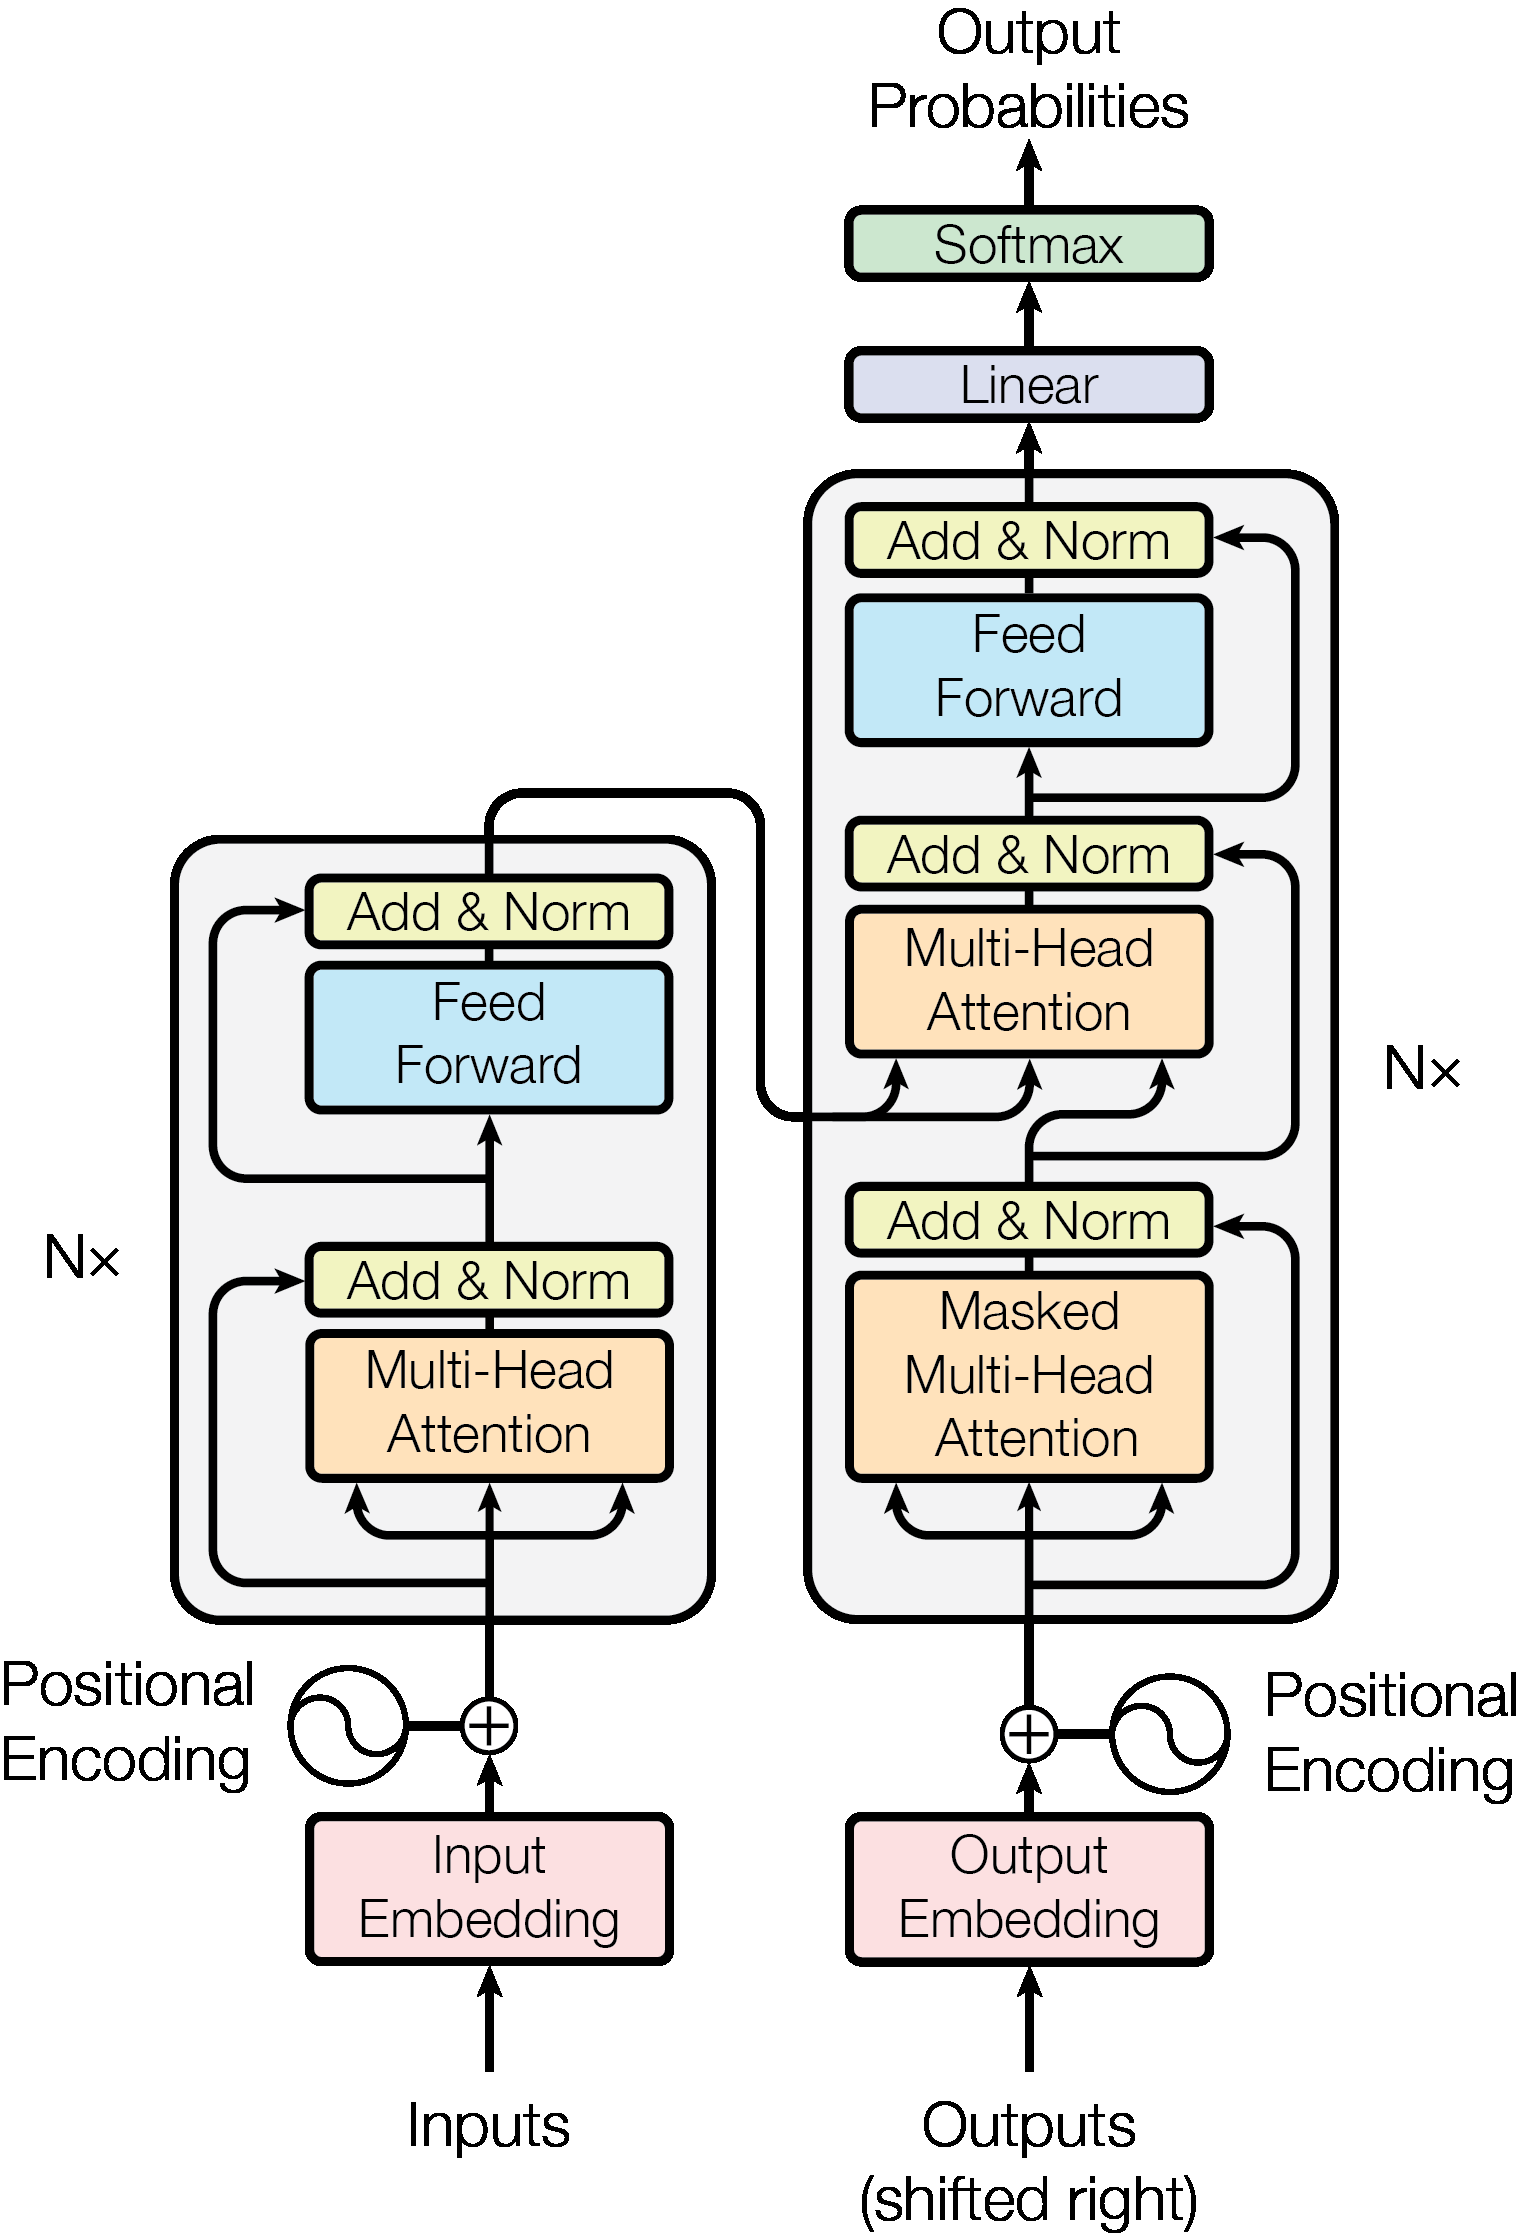
\includegraphics[height=6in]{figs/transformer.jpg}}
\caption[Transformer Architecture]{Transformer Architecture \cite{Vaswani2017}}
\label{fig:transformer_arch}
\end{figure}

\section{Integration of First Anticipation Experiments}

\subsection{Assembly Task: Build a Three-Color Flag \textcolor{red}{(Problem description: interaction experiment and focus on integration...)}}

\subsection{First Anticipation Experiments \textcolor{red}{(probabilities, rule-based \& rule-based + MediaPipe)}}

\textcolor{red}{The entire section below needs revising}

This chapter covers the implementation of the human-robot collaboration infrastructure that will serve as a base for an anticipation application. This includes the workflow of the different solutions, the general ROS architecture, and the details of the implemented state machine.

\subsection{Problem Description}

To develop the necessary infrastructure, a concrete problem was needed. For this work, it was chosen to use sequences of big \textcolor{red}{"Lego"} blocks comparable to the stripes of a flag, as shown in Fig~\ref{}.

\textcolor{red}{image with flags and blocks}

These blocks are initially placed behind the robot, and the robot must fetch them and place them next to the user so that the user can build a flag. The blocks must be fetched in a certain order and there must be a way for the user to tell the robot that it is fetching the wrong block.

\textcolor{red}{workspace from above}

\subsection{Solutions Workflow}

This subsection covers the workflow of the different solutions implemented.

\subsubsection{First Solution - Interaction Based}

The first version developed relied on interactions between the robot and the user. When the user puts his hand above a small block, if the state of the robot is $idle$, then it proceeds to fetch a block of the same colour. Additionally, when the user hovers his hand over the violet block while the state of the robot is $picking$ $up$ or $moving$ $closer$, it means that the robot fetched the wrong block, so it must stop and put the block back where it was before if it was already picked up.

The interactions in this solution are also the fallback behaviour if the methods in the following solutions fail to anticipate the block that the user desires.

\subsubsection{Second Solution - Probability Based}

The second version implemented consisted in having a database of probabilities that the robot would check to anticipate the block that the user would need next. These probabilities were established according to the possible country flags \textcolor{red}{(missing example)}. However, the first block is still requested by the user and, if the robot exhausts all possibilities that it knows of, the user is able to request the following block using the interactions described in the first solution.

\subsubsection{Third Solution - Rule Based}

\textcolor{red}{still need to explain this one}

\subsection{System ROS Architecture}

The communication between the robot, the sensors, and the programming logic is established using Robot Operating System (ROS) with the following 5 main nodes.

\textcolor{red}{a diagram might be a good idea to better visualize the solution}

\subsubsection{orbbec\_camera}

This node is responsible for receiving the color and depth images from the Orbbec camera and publishing them on ROS. In order to control to have better control over the lightness in the environment, the back-light compensation was raised to the maximum.

\subsubsection{human\_locator}

This node is responsible for analyzing the depth images and returning the position of the highest point in a certain region of interest which is then considered as the position of the human in the workspace.

\subsubsection{object\_color\_segmenter}

This node is responsible for analyzing the color images and returning the position of the objects in the workspace using color segmentation.

\subsubsection{decision\_making\_block}

This node is responsible for receiving the information resulting from the sensor data and keeping an internal state machine to decide what actions should be taken and when they should be taken.

\subsubsection{move\_it!}

This is a group of nodes responsible for planning the robot's trajectory in each action.

\subsection{State Machine Logic}

As said before, the decision\_making\_block node contains an internal state machine. Although the logic of some states changes depending on the solution, all implementations follow the same general design represented in the state machine diagram shown in Fig.~\ref{fig:state_machine}.

\begin{figure}[H]%[!ht]
    \centering
    \begin{tikzpicture}[
        > = stealth, % arrow head style
        shorten > = 1pt, % don't touch arrow head to node
        auto,
        node distance = 3.8cm, % distance between nodes
        thick % line style
    ]
    
    \tikzstyle{every state}=[
        draw = black,
        thick,
        fill = white,
        minimum size = 4mm,
        text width = 1.5cm,
        align = center
    ]
    
    \node[state] (idle) at (0,0) {idle};
    \node[state] (picking_up) [right of=idle] {picking up};
    \node[state] (moving_closer) [right of=picking_up] {moving closer};
    \node[state] (putting_down) [below of=picking_up] {putting down};
    \node[state] (stop_side_switch) [right of=moving_closer] {stop side switch};
    \node[state] (stop_wrong_guess) [above of=picking_up] {stop wrong guess};
    
    % \path[->] (idle) edge node[align=center] {received new\\sequence} (picking_up);
    % \path[->] (picking_up) edge node[align=center] {object\\picked up} (waiting);
    % \path[->] (waiting) edge node[align=center] {user\\finished} (moving_closer);
    % \path[->] (moving_closer) edge node[align=center] {robot in put\\down position} (putting_down);
    % \path[->] (putting_down) edge node[align=center] {object\\put down} (picking_up);
    % \path[->] (putting_down) edge[bend left] node[align=center] {sequence\\finished} (idle);
    % \path[->] (moving_closer) edge[bend left] node[align=center] {user changed\\side} (stop_side_switch);
    % \path[->] (stop_side_switch) edge[bend left] node[align=center] {robot\\stopped} (moving_closer);
    % \path[->] (picking_up) edge[bend right] node[align=center] {} (stop_wrong_guess);
    % \path[->] (waiting) edge node[align=center] {} (stop_wrong_guess);
    % \path[->] (moving_closer) edge[bend right] node[align=center] {wrong assembly\\sequence} (stop_wrong_guess);
    % \path[->] (stop_wrong_guess) edge[bend right] node[align=center] {reverted\\previous guess} (picking_up);

%Alternative lay-out for easier global configuration (vsantos)
\path[every edge,
	->,
	text width=1.8cm,
	align=center,
%	pos=0.4,
	]
(idle)             edge             node {knows which block is the next}   (picking_up)
(picking_up)       edge             node {object picked up}        (moving_closer)
(moving_closer)    edge[bend left]  node {robot in put down position} (putting_down)
(putting_down)     edge[bend left]  node {robot retreated}         (idle)
(moving_closer)    edge[bend left]  node {user changed side}       (stop_side_switch)
(stop_side_switch) edge[bend left]  node {robot stopped}           (moving_closer)
(picking_up)       edge             node[right] {wrong assembly sequence}                         (stop_wrong_guess)
(moving_closer)    edge[bend right]  node[above right] {wrong assembly sequence} (stop_wrong_guess)
(stop_wrong_guess) edge[bend right]  node[above left] {reverted previous guess} (idle)
; 
    
\end{tikzpicture}
    \caption{State Machine}
    \label{fig:state_machine}
\end{figure}

\begin{itemize}
    \item \textbf{idle}: State corresponding to when the robot does not know which is the next block. If the sequence has not started yet then it waits for the user to choose the first block and then the state changes to $picking$ $up$. If the sequence has already started then the database is fetched for the possible next blocks and then if at least one block is returned the state changes to $picking$ $up$ or if none is returned the system waits for the user to choose the next block.
    \item \textbf{picking up}: State corresponding to while the robot is picking up a certain block. After it picks it up the state changes to $moving$ $closer$ unless it was picking the wrong object in which case it changes to $stop$ $wrong$ $guess$.
    \item \textbf{moving closer}: State corresponding to the movement until the put-down position opposite to the user so that the robot does not constrain him. After the robot reaches the put-down position the state changes to $putting$ $down$. If the robot is holding the wrong object then the state changes to $stop$ $wrong$ $guess$ instead and if the user changes side the state changes to $stop$ $side$ $switch$.
    \item \textbf{putting down}: State corresponding to the movement necessary to put down the block in the table and the retreat of the robot outside the user's workspace. After that, the state changes to $idle$.
    \item \textbf{stop side switch}: State corresponding to the action of stopping the robot because the user changed sides. After the robot is stopped the state changes back to $moving$ $closer$.
    \item \textbf{stop wrong guess}: State corresponding to the action of stopping the robot because the user indicated that it was the wrong block. If the robot was already holding a block then that block is put back where it was while in this state. After the robot is stopped and it is not holding a block the state changes to $picking$ $up$ if there are still more possible blocks in the database. Otherwise, the state changes to $idle$ so that it waits for a user request.
\end{itemize}

\section{Final Remarks}